%Efficient computation
Dado que los problemas financieros son de corriente de datos, es decir, a
medida que avanza el tiempo aparecen nuevos ticks con información para el
modelo, no es posible incluir todos estos en un solo modelo.  Por lo tanto se
propone una versión online del VECM con la posibilidad de actualizar el modelo
con la nueva data y entregar respuestas en un corto perdiodo de tiempo (mínimo
menor a la frecuencia).

Obtener los vectores de cointegración usando el método de Johansen es también
un procedimiento costoso en cuanto a tiempo computacional. Sin embargo, como
los vectores de cointegración representan la relación a largo plazo entre
series de tiempo, no varian mucho en el tiempo. El algoritmo propuesto obtiene
nuevos vectores de cointegración solamente cuando la relación a largo plazo
cambia. Este cambio se detecta siguiendo en cada paso el cambio del \emph{Mean
Absolute Percentage Error} (MAPE) de los últimos n-ajustes del modelo.

Dado que VECM es un modelo basado en las series tiempo diferenciadas, el MAPE
es obtenido de $\Delta \mathbf{y}$ de la siguiente forma:

\begin{equation}\label{eq:MAPE}
\text{MAPE}[t] = \frac{1}{n} \sum_{i=1}^{n} \left| 
\frac{\Delta \mathbf{y}_{\text{true}}[t-i]-\Delta
\mathbf{y}_{\text{pred}}[t-i]}{\Delta \mathbf{y}_{\text{true}[t-i]}}
\right| \, , 
\end{equation}

\noindent donde $\Delta \mathbf{y}_{\text{true}}$ es el valor actual de la
serie de tiempo diferenciada $\mathbf{y}$ y $\Delta \mathbf{y}_{\text{pred}}$
es su predicción actual.

Cómo este número presenta un promedio el cual puede ser poco representativa de
la muestra se realiza además un estudio de las propiedades estadísticas
clásicas.

\section{Algoritmo Propuesto}

Se propone un algoritmo online con ventanas deslizantes para la predicción del
valor futuro de la cartera de stock FOREX usando el modelo VECM~\ref{alg:proposal}. 

\begin{algorithm}[h!]
\begin{algorithmic}[1]
\REQUIRE $\,$ \\
$\mathbf{y}$: Matriz con $N$ vectores de entrada y $l$ series de tiempo\\
$p$: número de valores anteriores \\
$L$: tamaño de la ventana deslizante ($L<N$) \\
$\text{mean\_error}$: MAPE umbral \\
$n$: puntos de interpolación para calcular el MAPE\\
\ENSURE  $\,$ \\
$\{\Delta \mathbf{y}_{\text{pred}}[L+1],\dots,\Delta \mathbf{y}_{\text{pred}}[N]\}$: predicciones del modelo
\FOR { $i =0$ to $N-L$ }
    \STATE $\mathbf{y}_i \gets \mathbf{y}[i:i+L]$
    \IF {i = 0 }
        \STATE{$v \gets \texttt{getJohansen}(\mathbf{y}_i,p)$}
        \STATE{$[\mathbf{A} \quad \mathbf{B}] \gets
        \texttt{vecMatrix}(\mathbf{y}_i,p,v)$}
    \ELSE
        \STATE{$[\mathbf{A} \quad \mathbf{B}] \gets
        \texttt{vecMatrixOnline}(\mathbf{y}_i,p,v,\mathbf{A},\mathbf{B})$}
        \STATE $\Delta \mathbf{Y}_{\text{true}}[i] \gets \mathbf{B}[-1,:]$
        \STATE $\Delta \mathbf{Y}_{\text{pred}}[i] \gets \mathbf{A}[-1,:] \times \mathbf{X}$
    \ENDIF
    \STATE $\mathbf{X} \gets \text{OLS} (\mathbf{A},\mathbf{B})$
    \STATE $\Delta \mathbf{y}_{\text{true}}[i] \gets \mathbf{B}[-n,:]$
    \STATE $\Delta \mathbf{y}_{\text{pred}}[i] \gets \mathbf{A}[-n,:] \times \mathbf{X}$
    \STATE $e \gets \texttt{mape}(\Delta \mathbf{y}_{\text{true}}, \Delta
    \mathbf{y}_{\text{pred}})$
    \IF {$\texttt{mean}(e) > \text{mean\_error}$}
        \STATE{$v \gets \texttt{getJohansen}(\mathbf{y}_i,p)$}
        \STATE{$\mathbf{A} \gets
        \texttt{vecMatrixUpdate}(\mathbf{y}_i,p,v,\mathbf{A})$}
        \STATE $\mathbf{X} \gets \texttt{OLS} (\mathbf{A},\mathbf{B})$
    \ENDIF
\ENDFOR
\STATE $\text{MAPE} \gets \texttt{mape}(\Delta \mathbf{Y}_{\text{true}}, \Delta
\mathbf{Y}_{\text{pred}})$
\end{algorithmic}
\caption{OVECM: Online VECM}
\label{alg:proposal}
\end{algorithm}

\noindent donde:

\begin{eqnarray}\label{eq:vecmatrix}
 \mathbf{A}&=&
   \begin{bmatrix} 
   \beta^\top \mathbf{y}_{p} & 
   \cdots & \beta^\top \mathbf{y}_{N-1} \\
   \Delta \mathbf{y}_p  & \cdots 
   &\Delta\mathbf{y}_{N-1} \\ 
   \vdots  & \ddots & \vdots \\
   \Delta\mathbf{y}_2  & \cdots 
   & \Delta \mathbf{y}_{N-p+1} \\
   1 & \cdots & 1 
   \end{bmatrix}^\top \label{eq:vecA} \, ,\\
\mathbf{B} & = &
 \begin{bmatrix}
 \quad\\
  \Delta \mathbf{y}_{p+1} & 
  \dots &
  \Delta \mathbf{y}_N \label{eq:vecB}\\
  \quad
 \end{bmatrix}^\top \, ,\\
\mathbf{X}&=&
  \begin{bmatrix}
   \quad \\
   \alpha & \phi_1^* & \cdots & \phi_{p-1}^* & \mathbf{c} \\  
   \quad
   \end{bmatrix}^\top \, ,\\
\mathbf{E} &=&
\begin{bmatrix}
   \quad \\
   \mathbf{\epsilon}_{p+1} &
   \dots &
   \quad &\mathbf{\epsilon}_N \, \\ \quad
\end{bmatrix}^\top 
\end{eqnarray}

La propuesta considera lo siguiente:
\begin{itemize}
 \item La función \texttt{getJohansen} retorna los vectores de cointegración
dados por el método de johansen considerando el test estadístico \emph{trace}
al 95\% de nivel de significancia.
 \item La función \texttt{vecMatrix} retorna las matrices~(\ref{eq:vecA})
y~(\ref{eq:vecB}) que permiten resolver el VECM.
 \item La función \texttt{vecMatrixOnline} retorna las matrices~(\ref{eq:vecA})
y~(\ref{eq:vecB}) agregando la nueva data y removiendo la antigua, evitando
calcular la matriz $\mathbf{A}$ desde cero.
 \item El modelo se resuelve usando OLS.
 \item La función \texttt{mape} obtiene el MAPE dentro de la muestra
(interpolación) para la serie de tiempo $l$.
 \item Los vectores de cointegración se obtienen al comienzo y se actualizan
cuando el promedio de todos los MAPEs en la variable $e$ es superior a cierto
error dado por el umbral definido.
 \item Si se requieren nuevos vectores de cointegración, la función
\texttt{vecMatrixUpdate} solo actualiza las columnas correspondientes de la
matriz $\mathbf{A}$ afectados por esos vectores(mirar la
ecuación~\ref{eq:vecA})
\end{itemize}

La propuesta fue comparada contra la versión modificada VECM que solo considera
datos en una ventana deslizante (SLVECM). Esto se realizo para comparar los
tiempos de ejecución. En SLVEM la función \texttt{getJohansen} y
\texttt{vecMatrix} es llamada en cada iteración. El algoritmo ~\ref{alg:SLVECM}
muestra la modificación.

\begin{algorithm}[ht]
\begin{algorithmic}[1]
\REQUIRE $\,$ \\
$\mathbf{y}$: matrix con $N$ vectores de entrada y $l$ series de tiempo\\
$p$: número de valores anteriores\\
$L$: tamaño de la ventana deslizante ($L<N$) \\
\ENSURE  $\,$ \\
$\{\Delta \mathbf{y}_{\text{pred}}[L+1],\dots,\Delta \mathbf{y}_{\text{pred}}[N]\}$: predicciones del modelo
\STATE{$v \gets \texttt{getJohansen}(\mathbf{y}[:L],p)$}
\FOR { $i =0$ to $N-L$ }
    \STATE $\mathbf{y}_i \gets \mathbf{y}[i:i+L]$
    \STATE{$[\mathbf{A} \quad \mathbf{B}] \gets
    \texttt{vecMatrix}(\mathbf{y}_i,p,v)$}
    \IF {$i > 0$}
        \STATE $\Delta \mathbf{Y}_{\text{true}}[i] \gets \mathbf{B}[-1,:]$
        \STATE $\Delta \mathbf{Y}_{\text{pred}}[i] \gets \mathbf{A}[-1,:] \times \mathbf{X}$
    \ENDIF
    \STATE{$v \gets \texttt{getJohansen}(\mathbf{y}_i,p)$}
    \STATE{$[\mathbf{A} \quad \mathbf{B}] \gets
    \texttt{vecMatrix}(\mathbf{y}_i,p,v)$}
    \STATE $\mathbf{X} \gets \text{OLS} (\mathbf{A},\mathbf{B})$
\ENDFOR
    \STATE $\text{MAPE} \gets \texttt{mape}(\Delta \mathbf{Y}_{\text{true}}, \Delta
    \mathbf{Y}_{\text{pred}})$
\end{algorithmic}
\caption{SLVECM: Sliding window VECM}
\label{alg:SLVECM}
\end{algorithm}

Ambos algoritmos entregan el MAPE de la predicción fuera de la muestra. Es
importante destacar que OVECM con mean\_error=0 entregará los mismos MAPE que
SLVEM.

\section{Parámetros del algoritmo}
Cómo se puede desprender de la formulación matemática de los modelos, hay dos
parámetros que deben ser definidos: largo de la ventana (L), cantidad de lags
(P). Existen variados métodos para la estimación de parámetros, sin embargo se
usará el criterio de información de Akaike Information Criterion.

\subsection{Criterio de información de Akaike}
El Criterio de información de Akaike (AIC por sus siglas en inglés) fue
inicialmente desarrollado en series temporales \emph{citar}. Su idea clave es
la de penalizar un exceso de parámetros ajustados para cierto modelo. El AIC es
un estimador muestral de $E[ln(f(X|\theta)]$, esperanza de la log-verisimilitud
(o negantropìa) que viene dado por la expresión~\ref{eq:aicformula}:

\begin{equation}
\label{eq:aicformula}
AIC = \underset{\text{bias}}{-\frac{2l}{N}} + 
\underset{\text{variance}}{\frac{2k}{N}}
\end{equation}

\noindent donde

\begin{description}
\item[l] es la función verosimilitud
\item[k] número de parámetros ajustados (incluyendo la varinza)
\item[N] número de observaciones
\end{description}

Se calcula el valor de AIC para cada modelo con el mismo set de datos, y
el \emph{mejor} modelo es el que tiene menor valor de AIC.
El primer término de AIC puede ser interpretado como una medida de la bondad
del ajuste, mientras el segundo término es una penalización, creciente conforme
aumenta el número de parámetros, de acuerdo al Principio de
Parsimonia~\ref{fig:parsimony}. El AIC enfatiza la bondad del modelo, sin
embargo no pretende identificar el modelo verdadero. Que un modelo sea el que
mejor ajusta a los datos, no quiere decir que sea el modelo real o verdadero.
Más bien, significa que el modelo es el mejor entre los modelos candidatos, en
el sentido que proporciona la aproximación más cercana a la realidad o al
verdadero modelo. El modelo que mejor se ajusta a los datos, podría cambiar
mucho en función del tamaño muestral, como en el caso de los polinomios
interpoladores.

\begin{figure}[h!t]
    \begin{center}
        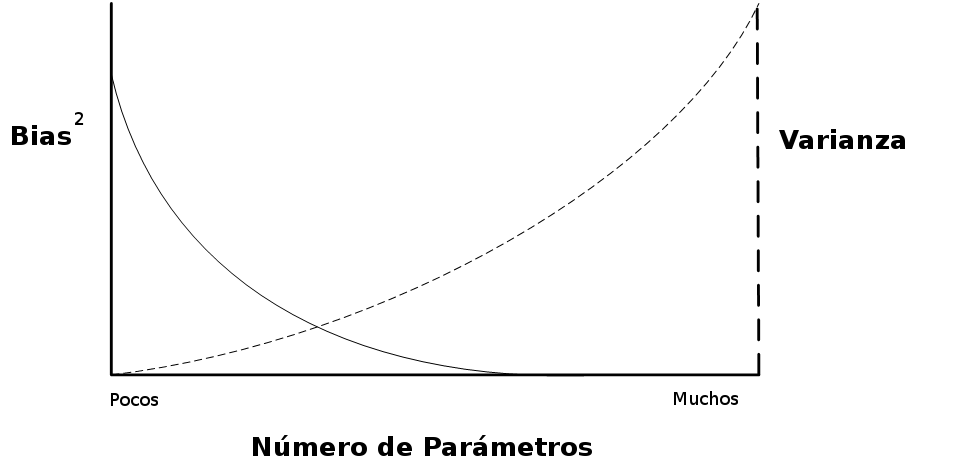
\includegraphics[width=0.8\textwidth]{images/parsimony}
        \caption{Principio de Parsimonia}
        \label{fig:parsimony}
    \end{center}
\end{figure}

Algunas de las ventajas del AIC que lo hacen tan utilizado en la práctica, son
su simplicidad (no requiere acudir a ninguna tabla para observar el valor
correspondiente) y facilidad para ser implementado, y el hecho de que no existe
el problema de especificar subjetivamente un nivel de significación arbitrario
para contrastar dos modelos.

\section{Diagrama de Clases}
La implementación fue realizada en Python, usando principalmente las bibliotecas:
\begin{itemize}
 \item Pandas: biblioteca para manipulación y análisis de datos.
\footnote{\url{http://pandas.pydata.org}}
 \item Statsmodels: módulo que permite explorar data, estimar modelos y test
estadísticos \footnote{\url{http://statsmodels.sourceforge.net/}}.
 \item Numpy: paquete de computación científica en Python, provee estructuras
de datos y funciones de álgebra lineal entre otras cosas.
\footnote{\url{http://www.numpy.org}}
 \item CULA: es un set de librerías de algebra lineal usando
GPU\footnote{\url{http://www.culatools.com/}}.
 \item Scikit.CUDA: provee interfaces a un set de funciones de CUDA, cuBLAS y
otras bibliotecas. La idea es poder ejecutar funciones de cuda desde python a
través de wrappers. \footnote{\url{http://scikits.appspot.com/cuda}}
\end{itemize}

Basándose en esas bibliotecas y otras más, se crearon 3 clases mostrados en la
figura \ref{fig:class_diagram}:
\begin{itemize}
 \item Util: provee métodos generales utilizados por las otras 2 clases.
 \item Reader: clase que lee los datos ticks desde archivos CSV descargados
desde dukascopy, provee funciones para juntar monedas en la misma estructura de
datos, hacer resampling a cierta frecuencia y normalizar monedas, entre otras
funciones.
 \item Matrix: es la clase es más extensa y contiene los principales métodos
utilizados por los algoritmos, entre ellos la creación de las matrices VAR y
VECM, el update de las matrices optimizado para la ventana deslizante, cálculo
de vectores de integración mediante Johansen, test de estacionaridad usando
Augmented Dicky Fuller, Errores porcentuales, etc.
\end{itemize}

\begin{figure}[h!t]
    \begin{center}
        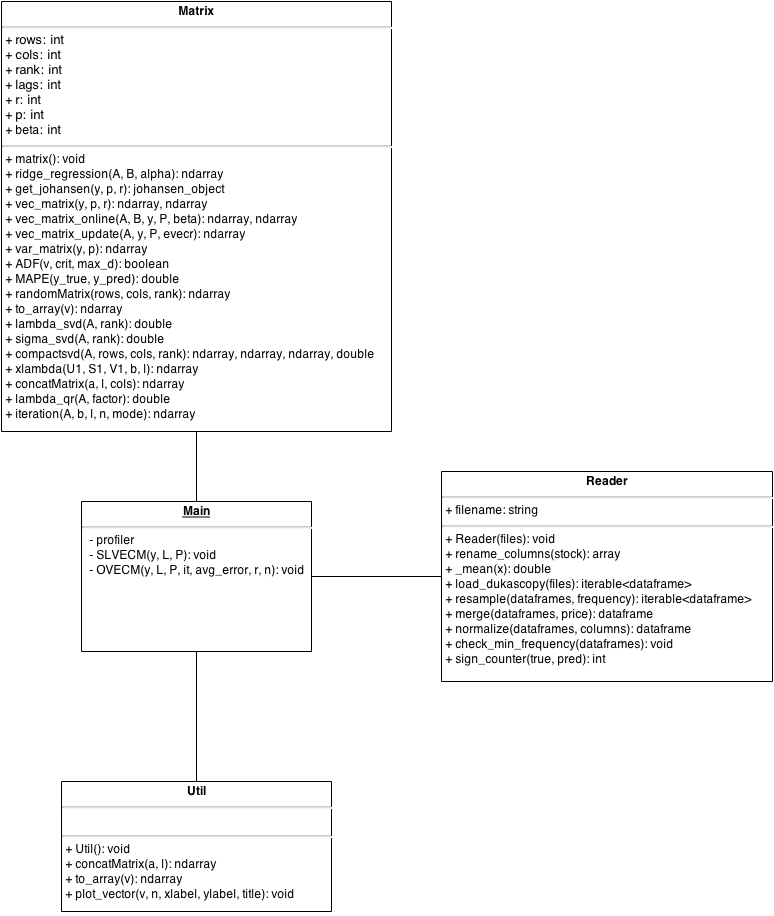
\includegraphics[width=0.8\textwidth]{images/class_diagram.png}
        \caption{Diagrama de Clases}
        \label{fig:class_diagram}
    \end{center}
\end{figure}

%\section{Métodos a paralelizar}
